\PassOptionsToPackage{unicode=true}{hyperref} % options for packages loaded elsewhere
\PassOptionsToPackage{hyphens}{url}
\PassOptionsToPackage{dvipsnames,svgnames*,x11names*}{xcolor}
%
\documentclass[
  12pt,
]{report}
\usepackage{lmodern}
\usepackage{setspace}
\setstretch{1.5}
\usepackage{amssymb,amsmath}
\usepackage{ifxetex,ifluatex}
\ifnum 0\ifxetex 1\fi\ifluatex 1\fi=0 % if pdftex
  \usepackage[T1]{fontenc}
  \usepackage[utf8]{inputenc}
  \usepackage{textcomp} % provides euro and other symbols
\else % if luatex or xelatex
  \usepackage{unicode-math}
  \defaultfontfeatures{Scale=MatchLowercase}
  \defaultfontfeatures[\rmfamily]{Ligatures=TeX,Scale=1}
\fi
% use upquote if available, for straight quotes in verbatim environments
\IfFileExists{upquote.sty}{\usepackage{upquote}}{}
\IfFileExists{microtype.sty}{% use microtype if available
  \usepackage[]{microtype}
  \UseMicrotypeSet[protrusion]{basicmath} % disable protrusion for tt fonts
}{}
\makeatletter
\@ifundefined{KOMAClassName}{% if non-KOMA class
  \IfFileExists{parskip.sty}{%
    \usepackage{parskip}
  }{% else
    \setlength{\parindent}{0pt}
    \setlength{\parskip}{6pt plus 2pt minus 1pt}}
}{% if KOMA class
  \KOMAoptions{parskip=half}}
\makeatother
\usepackage{xcolor}
\IfFileExists{xurl.sty}{\usepackage{xurl}}{} % add URL line breaks if available
\IfFileExists{bookmark.sty}{\usepackage{bookmark}}{\usepackage{hyperref}}
\hypersetup{
  pdftitle={Development \& Application of a Closed-Loop Continuous Optical Neural Interface},
  pdfauthor={Mark Bucklin},
  pdfkeywords={session types, applied type system, dependent types, linear types, multirole logic},
  colorlinks=true,
  linkcolor=Maroon,
  filecolor=Maroon,
  citecolor=Blue,
  urlcolor=Blue,
  breaklinks=true}
\urlstyle{same}  % don't use monospace font for urls
\usepackage{color}
\usepackage{fancyvrb}
\newcommand{\VerbBar}{|}
\newcommand{\VERB}{\Verb[commandchars=\\\{\}]}
\DefineVerbatimEnvironment{Highlighting}{Verbatim}{commandchars=\\\{\}}
% Add ',fontsize=\small' for more characters per line
\newenvironment{Shaded}{}{}
\newcommand{\AlertTok}[1]{\textcolor[rgb]{1.00,0.00,0.00}{\textbf{#1}}}
\newcommand{\AnnotationTok}[1]{\textcolor[rgb]{0.38,0.63,0.69}{\textbf{\textit{#1}}}}
\newcommand{\AttributeTok}[1]{\textcolor[rgb]{0.49,0.56,0.16}{#1}}
\newcommand{\BaseNTok}[1]{\textcolor[rgb]{0.25,0.63,0.44}{#1}}
\newcommand{\BuiltInTok}[1]{#1}
\newcommand{\CharTok}[1]{\textcolor[rgb]{0.25,0.44,0.63}{#1}}
\newcommand{\CommentTok}[1]{\textcolor[rgb]{0.38,0.63,0.69}{\textit{#1}}}
\newcommand{\CommentVarTok}[1]{\textcolor[rgb]{0.38,0.63,0.69}{\textbf{\textit{#1}}}}
\newcommand{\ConstantTok}[1]{\textcolor[rgb]{0.53,0.00,0.00}{#1}}
\newcommand{\ControlFlowTok}[1]{\textcolor[rgb]{0.00,0.44,0.13}{\textbf{#1}}}
\newcommand{\DataTypeTok}[1]{\textcolor[rgb]{0.56,0.13,0.00}{#1}}
\newcommand{\DecValTok}[1]{\textcolor[rgb]{0.25,0.63,0.44}{#1}}
\newcommand{\DocumentationTok}[1]{\textcolor[rgb]{0.73,0.13,0.13}{\textit{#1}}}
\newcommand{\ErrorTok}[1]{\textcolor[rgb]{1.00,0.00,0.00}{\textbf{#1}}}
\newcommand{\ExtensionTok}[1]{#1}
\newcommand{\FloatTok}[1]{\textcolor[rgb]{0.25,0.63,0.44}{#1}}
\newcommand{\FunctionTok}[1]{\textcolor[rgb]{0.02,0.16,0.49}{#1}}
\newcommand{\ImportTok}[1]{#1}
\newcommand{\InformationTok}[1]{\textcolor[rgb]{0.38,0.63,0.69}{\textbf{\textit{#1}}}}
\newcommand{\KeywordTok}[1]{\textcolor[rgb]{0.00,0.44,0.13}{\textbf{#1}}}
\newcommand{\NormalTok}[1]{#1}
\newcommand{\OperatorTok}[1]{\textcolor[rgb]{0.40,0.40,0.40}{#1}}
\newcommand{\OtherTok}[1]{\textcolor[rgb]{0.00,0.44,0.13}{#1}}
\newcommand{\PreprocessorTok}[1]{\textcolor[rgb]{0.74,0.48,0.00}{#1}}
\newcommand{\RegionMarkerTok}[1]{#1}
\newcommand{\SpecialCharTok}[1]{\textcolor[rgb]{0.25,0.44,0.63}{#1}}
\newcommand{\SpecialStringTok}[1]{\textcolor[rgb]{0.73,0.40,0.53}{#1}}
\newcommand{\StringTok}[1]{\textcolor[rgb]{0.25,0.44,0.63}{#1}}
\newcommand{\VariableTok}[1]{\textcolor[rgb]{0.10,0.09,0.49}{#1}}
\newcommand{\VerbatimStringTok}[1]{\textcolor[rgb]{0.25,0.44,0.63}{#1}}
\newcommand{\WarningTok}[1]{\textcolor[rgb]{0.38,0.63,0.69}{\textbf{\textit{#1}}}}
\usepackage{graphicx,grffile}
\makeatletter
\def\maxwidth{\ifdim\Gin@nat@width>\linewidth\linewidth\else\Gin@nat@width\fi}
\def\maxheight{\ifdim\Gin@nat@height>\textheight\textheight\else\Gin@nat@height\fi}
\makeatother
% Scale images if necessary, so that they will not overflow the page
% margins by default, and it is still possible to overwrite the defaults
% using explicit options in \includegraphics[width, height, ...]{}
\setkeys{Gin}{width=\maxwidth,height=\maxheight,keepaspectratio}
\setlength{\emergencystretch}{3em}  % prevent overfull lines
\providecommand{\tightlist}{%
  \setlength{\itemsep}{0pt}\setlength{\parskip}{0pt}}
\setcounter{secnumdepth}{5}
% Redefines (sub)paragraphs to behave more like sections
\ifx\paragraph\undefined\else
  \let\oldparagraph\paragraph
  \renewcommand{\paragraph}[1]{\oldparagraph{#1}\mbox{}}
\fi
\ifx\subparagraph\undefined\else
  \let\oldsubparagraph\subparagraph
  \renewcommand{\subparagraph}[1]{\oldsubparagraph{#1}\mbox{}}
\fi

% set default figure placement to htbp
\makeatletter
\def\fps@figure{htbp}
\makeatother

\begin{itemize}
\item
  \usepackage{appendix}
\item
  \usepackage{caption}
\item
  \usepackage{float}
\item
  \numberwithin{figure}{section}
\item
  \numberwithin{table}{section}
\item
  \numberwithin{equations}{section}
\item
  \pagenumbering{arabic}
\item
  \setstretch{1}
\item
  \setlength{\parskip}{9pt}
\end{itemize}
\makeatletter
\@ifpackageloaded{subfig}{}{\usepackage{subfig}}
\@ifpackageloaded{caption}{}{\usepackage{caption}}
\captionsetup[subfloat]{margin=0.5em}
\AtBeginDocument{%
\renewcommand*\figurename{Figure}
\renewcommand*\tablename{Table}
}
\AtBeginDocument{%
\renewcommand*\listfigurename{List of Figures}
\renewcommand*\listtablename{List of Tables}
}
\@ifpackageloaded{float}{}{\usepackage{float}}
\floatstyle{ruled}
\@ifundefined{c@chapter}{\newfloat{codelisting}{h}{lop}}{\newfloat{codelisting}{h}{lop}[chapter]}
\floatname{codelisting}{Listing}
\newcommand*\listoflistings{\listof{codelisting}{List of Listings}}
\makeatother

\title{Development \& Application of a Closed-Loop Continuous Optical Neural
Interface}
\author{Mark Bucklin}
\date{April 13, 2017}

\begin{document}
\maketitle
\begin{abstract}
abstract
\end{abstract}

{
\hypersetup{linkcolor=}
\setcounter{tocdepth}{2}
\tableofcontents
}
\listoftables
\listoffigures
\hypertarget{introduction-background-and-literature-review}{%
\chapter{Introduction: Background and Literature
Review}\label{introduction-background-and-literature-review}}

\hypertarget{primary-goals}{%
\section{Primary Goals}\label{primary-goals}}

The function of the brain is to translate/encode sensory input into
neural output, actuating an effect that promotes organism survival or
the survival of offspring. It achieves this by communicating input
through interconnected neurons via converging and diverging connections
that comprise the neural network. One way to study the brain is by
testing and observing the properties of individual neurons and the
response to changing conditions at the direct connections they form with
others. Another approach is to observe a collection of neurons and
measure their response to variable conditions in their external
environment either by recording or stimulating variations in sensory
input or measuring an organism's physical/behavioral response.

One might presume that the expansion of information provided by
measuring activity from a larger number of cells in a network would
simplify analysis in stimulus-response type experiments and afford
insight about underlying functional mechanisms. Unfortunately, the
correlation and information theoretic procedures traditionally used to
make these associations suffer from a systematic bias that exponentially
grows with the number responses considered for each stimulus (i.e., the
number of included cells). The trial number necessary to overcome this
bias becomes exponentially large although methods such as
shuffling/resampling tests exist for bias correction.

A systems neuroscience experiment benefits from online feedback in one
or both of two ways:

\begin{enumerate}
\def\labelenumi{\arabic{enumi}.}
\item
  It informs the user regarding the current number of trials, i.e.,
  repeated presentations of the stimulus will be sufficient to overcome
  limited sampling bias in an experiment attempting to learn the neural
  response/pattern associated with a specific stimulus. This could be
  done by testing pattern hypotheses online against subsets of collected
  data and then assessing their stability.
\item
  Online pattern recognition feedback maximizes the information in the
  response to a stimulus either by directing modification of the
  stimulus, or directing modification of the field-of-view either by
  directing modification of the stimulus, or directing modification of
  the field-of-view.
\end{enumerate}

Streaming processing addresses the issues of processing and storing for
sufficient learning from large networks. Additionally, I propose a
strategy in the methods section by which incorporating this online
processing stream into stimulus-response-type experiments could help
correct limited sampling bias, enabling neural coding analysis in large
populations of neurons (Ince et al. 2009). This approach works when the
experimental intention is to study neural coding in general, for which
it's sufficient to have an arbitrary stimulus.

An additional goal of this project focuses on the ability to use the
expanded information made available by the first two project components
to train an encoder that predicts intended motor states from one healthy
mouse and uses the predictions to direct neuromodulatory control of a
second mouse. This setup simulates pathologic disconnection in a brain,
tests the ability to distinguish intention to start or stop running, and
also applies this is a manner that easily measures performance.

\hypertarget{optical-imaging-of-neural-activity}{%
\section{Optical Imaging of Neural
Activity}\label{optical-imaging-of-neural-activity}}

Optical techniques for observing neural activity have recently advanced
owing to both an evolution of digital imaging technology, and the
development of engineered proteins that act as fluorescent indicators of
neural activity. Image sensors, like those found in scientific-CMOS
(sCMOS) cameras are larger, faster, and more sensitive than prior
scientific grade cameras. Meanwhile, the latest generation of
Genetically Encoded Calcium Indicators (GECIs), collectively called
GCaMP6, report fluctuations in neural activation with extremely high
fidelity. This combination of developments enables neuroscientists to
open a wider channel to the brain than previously possible using
conventional epifluorescence microscopy techniques that enable
simultaneous recording from hundreds to thousands of neurons. Expanding
the fraction of the observable neurons in an interconnected network
could improve understanding of neural coding and provide insight into
mechanistic properties of neural disease. Additionally, feeding a large
set of neural response information to a machine learning algorithm in a
neuroprosthetic application may provide improved predictive performance
even when the exact mechanism of prediction is difficult to discern.
However, several major challenges currently antagonize the potential
benefits of these new technologies:

\begin{enumerate}
\def\labelenumi{\arabic{enumi}.}
\tightlist
\item
  The increased size of raw data from a single imaging session can
  easily overwhelm the computational resources typically used to process
  similar but smaller sets of data.
\item
  The accumulation of raw data on disk over multiple imaging sessions
  quickly exceeds the data-storage capacity of most lab-scale servers,
  forcing researchers to halt data collection to process and delete,
  potentially creating a ``nightmare scenario''.
\item
  The experimental design and data analysis procedures familiar to
  neuroscientists for network activity data for 5 to 10 cells produce
  highly biased spurious results in the absence of numerous
  stimulus-response repetitions, i.e., trials. The number of repeated
  trials sufficient to produce an accurate description of the neural
  response to any stimulus is on the order of 2N, where N is the number
  of neurons being measured.
\end{enumerate}

In the chapters that follow I provide background on the general
procedure for offline video processing. I also discuss some of the
issues that limit execution of these procedures on a large dataset, and
the variety of approaches that I and others have attempted to address
this issue. I then introduce the streaming approach that is capable of
directly processing video during acquisition and extracting signals,
thereby saving relevant signals only while also discarding or
compressing the raw video. This approach relies on GPU programming and
therefore I also provide background on the application of graphics cards
for computationally demanding tasks. Using a graphics card for
programming in the MATLAB environment is also discussed.

Capturing wide-field fluorescence images at high spatial and temporal
resolution enables us to measure functional dynamic changes in multiple
cells within a large interconnected network. Extracting a measure for
each cell in a way that preserves spatial and temporal continuity with
uniform/unbiased sampling of the observed signal is achievable but
several factors complicate procedures intended to accomplish this task.
One class of computer-vision procedure commonly applied to this task is
image-segmentation (cell-segmentation in histology applications), a
procedure that attempts to represent distinct objects in an image by
association of each image pixel with one of any number of abstract
objects or with the background. A variety of algorithms exist for
efficiently performing this operation on single images. Most methods can
be extended to operate in a 3rd dimension, applied to stacks of image
frames to enable tracking cells at multiple depths, or equivalently over
time.

However, motion induced by physiologic changes and animal movement
necessitates the correct alignment of all frames in the sequence.
Moreover, the massive fluctuations in signal intensity from individual
and spatially overlapping cells often breeds unstable solutions for
alignment that radically complicate cell identification routines by
disrupting temporal continuity. Implementing a reliable procedure for
identifying and tracking the same cells in each frame throughout the
sequence thus becomes non-trivial.

\hypertarget{procedures-for-calcium-imaging}{%
\section{Procedures for Calcium
Imaging}\label{procedures-for-calcium-imaging}}

The general goal of processing image data from functional fluorescence
imaging experiments is to restructure raw image data in a way that maps
pixels in each image frame to distinct individual cells or subcellular
components, called `Regions-Of-Interest' (ROI). Pixel-intensity values
from mapped pixels are often reduced by combination to single
dimensional `trace' time-series. These traces indicate the fluorescence
intensity of an individual neuron over time, and the collection
approximates the distinct activity of all individual neurons in the
microscope's field of view. However, this task is made difficult by
motion of the brain throughout the experiment and by the apparent
overlap of cells in the single image plane due to limitations of the
camera's 2-dimensional perspective. These issues can be partially
mitigated with a few image pre-processing steps. Most importantly is the
alignment of images to correct for motion. These options are described
in the Methods \& Approaches section below. Most software packages
specifically geared toward functional imaging implement either of two
basic classes of pixel-\textgreater{}cell mapping algorithms. One
approach is to use image-segmentation routines for computer vision that
seeks to combine adjacent pixels into distinct spatially segregated
regions representing objects in the image.

The other common approach is to perform an eigenvalue decomposition on
the covariance matrix from a stack of image frames (also called spectral
decomposition, or Principal Component Analysis, PCA), resulting in an
assembly of basis vectors that define the weighting coefficients for
each pixel. Multiplying the basis-vectors (i.e., ``components'') with
all frames produces a one-dimensional trace for each component. The
linear combination is similar to the weighted image-segmentation method
in that it assigns fractional coefficients to pixels. However, the
procedure for computing the covariance matrix employed by PCA operates
on as many pixels as exist in the image, multiplying each with every
other pixel that creates a problem with np2 complexity, where p is the
number of pixels in the image. I mention these issues inherent to PCA
not because this project addresses them but because this project was
initiated following substantial difficulty attempting to use PCA-based
cell sorting methods with large datasets.

\hypertarget{computer-software-environments-for-image-processing}{%
\section{Computer Software Environments for Image
Processing}\label{computer-software-environments-for-image-processing}}

The widespread usage of MATLAB in neuroscience communities lends
potential for greater usability and easier adaptation to software
developed in this environment. While software development environments
focused on ``ease-of-use'' traditionally presume crippling sacrifices to
computational performance, this assumption is now less accurate.

Standard programs include ImageJ, the built-in routines in MATLAB's
Image Processing Toolbox, Sci-Kits Image for Python, and a remarkable
diversity of miscellaneous applications. MATLAB is a commercial software
development platform that is geared toward fast production and the
prototyping of data processing routines in a high-level programming
language. It implements several core libraries (LINPACK, BLAS, etc.)
that make multi-threaded operations on matrix type data highly
efficient. While MATLAB has traditionally been considered the standard
across neuroscience research labs, it is well recognized that its
performance was lackluster for ``vectorized'' routines as compared to
applications developed using lower-level languages like FORTRAN, C, and
C++. Nevertheless, it remained in common use, and recent releases have
added features that can drastically mitigate its poor performance
issues, particularly through the development of a ``Just-In-Time''
compiler that automatically optimizes the deployment of computation
accelerator resources for standard MATLAB functions. This feature
enables code that performs repeated operations using for-loops or
while-loops nearly as fast as equivalent code written in C.
Additionally, code can be compiled into executable format using the
Matlab Compiler toolbox, or used to generate equivalent C or C++ code
using Matlab Coder.

\hypertarget{computational-resources-for-processing-large-data-sets}{%
\section{Computational Resources for Processing Large Data
Sets}\label{computational-resources-for-processing-large-data-sets}}

Routines for extracting the activity in each cell from a collection of
raw imaging data rely on simultaneous access to many pixels separated
over space and time (and consequently, are separated on a disk). For
long recording sessions however, the size of the collection of stored
image data dramatically grows. This substantial increase in data size
easily exceeds the capacity of system memory in the typical workstation
computer available to most researchers. Thus, performing the necessary
processing performance enhancing routines using standard programs is
often unfeasible.

Another popular approach to this challenge is the migration of
processing routines to a cluster-based system. In this way, image data
can be distributed across many interconnected computer nodes capable of
performing all locally restricted image processing procedures in
parallel and then passing data to other nodes in the cluster for tasks
that rely on comparisons made across time. Access to clusters capable of
performing in this way has been historically restricted to researchers
in universities or other large organization, and the diversity of
cluster types is sizeable, with clusters often having very particular
configuration requirements for efficiently implementing data processing
jobs. These issues pose difficulty to the use and shared development of
software libraries for image processing routines, although the growth of
``cloud computing'' services such as Amazon's EC2 and the Google Compute
Engine, as well as collaborative computing facilities such as the
Massachusetts Green High-Performance Computing Center minimize several
of these processing issues. Additionally, efforts to produce a
standardized interface for accessing and distributing data and for
managing computing resources across diverse computing environments have
seen appreciable success. Apache's release of the open-source cluster
computing framework, Hadoop, and a companion data-processing engine
called Spark, has encouraged a massive growth in collaborative
development projects, a consequently increased the availability of
robust shared libraries for data processing in a variety of
applications. The Spark API can be accessed using the open-source
programming Python or other languages including Java, Scala, or R. The
Thunder library, a Spark package released by the Freeman lab and
developed in collaboration with a number of other groups at Janelia Farm
and elsewhere is specifically geared for image processing of neural
imaging data.

Many applications will find that the recent improvements in
accessibility and standardization make cluster computing an attractive
and worthwhile option for processing large sets of reusable data.
However, this strategy imposes harsh limitations for a neuroscientist
engaged in a project that is continuously generating new data, as the
time required to transfer entire imaging data sets across the internet
may be prohibitive. Unfortunately, storage on the cloud is not so
unlimited that it can manage an accumulated collection of imaging data
generated that approximates the rate that at which sCMOS cameras
operate. This rate imbalance is a central motivating issue in this
project and is discussed in detail below.

The generation of sCMOS cameras available at the start of this work
capture full-frame resolution video at either 30 fps or 100 fps
depending on the data interface between camera and computer (USB3.0 or
CameraLink). At 16-bits per pixel and 2048x2048 pixels, the maximum data
rate for the USB3.0 camera is 240 MB/s. Imaging sessions typically last
30-minutes or less. Pixels are typically binned down 2x2, and frame rate
is often reduced to work within the constraints our laboratory
workstations impose on processing speed and storage. However, the effect
of doubling resolution on processing time when using the graphics card
is virtually negligible. Identifying ROIs online and extracting the
traces of neural activity allows us to discard acquired images and
instead, only store the relevant pixels for later analysis.

\hypertarget{graphics-processing-units-for-video-processing}{%
\subsection{Graphics Processing Units for Video
Processing}\label{graphics-processing-units-for-video-processing}}

Graphics Processing Units were traditionally developed for the consumer
gaming market. They are optimized for the process that involves
translating a continuous stream of information into a two-dimensional
image format for transfer to a computer monitor. In the context of
gaming, the stream of information received by a GPU describes the state
of objects in a dynamic virtual environment and is typically produced by
a video game engine. These processors are highly optimized for this
task. However, they are equally efficient at performing the same
procedure type in reverse, reducing a stream of images to structured
streams of information about dynamic objects in the image. These
features render them popular for video processing and computer vision
applications.

All GPU architectures consists of a hierarchy of parallel processing
elements. NVIDIA's CUDA architecture refers to the lowest level
processing element as ``CUDA Cores'' and the highest level as
``Symmetric Multiprocessors.'' Typically, data is distributed across
cores and multiprocessors by specifying a layout in C-code using
different terminology, ``threads'' and ``blocks.'' Blocks are then
termed to be organized in a ``grid.'' Adapting traditional image
processing or computer vision algorithms to quickly run on a GPU
involves efficiently distributing threads and ideally minimizes
communication between blocks.

MATLAB makes processing data using the GPU seemingly trivial by
overloading a large number of built in functions. Performance varies
however. Writing a kernel-type subfunction is often the fastest way to
implement a routine written as if it operates on single (scalar) element
only that can be called on all pixels at once or employs all
pixel-subscripts used by the function to retrieve the pixel value at a
given subscript. The kernel-type function is compiled into a CUDA kernel
the first time it's called, then repeated calls directly contact the
kernel with minimal overhead. Calls typically use the arrayfun()
function.

Data transfers between system memory and graphics memory is often a
major bottle-neck. Therefore, this operation is best performed only
once. However, once data is available to the GPU, many complex
operations can be performed to extract information from the image
without exceeding the processing-time limit imposed by the frame-rate of
the camera sending the images.

In total, this project employs advances in both software and hardware
that facilitate rapid accurate image analysis of living organisms with
the ultimate goals of simplifying the acquisition and analysis of neural
activity indicators in both normal and pathologic states.

\hypertarget{neural-interfaces-fabrication-programming-and-assembly}{%
\chapter{Neural Interfaces: Fabrication, programming, and
assembly}\label{neural-interfaces-fabrication-programming-and-assembly}}

This chapter describes several projects that were started early during
my graduate studies. Each project is similar in that they are outside
the realm of optical imaging of neural activity, which is the focus of
the rest of this dissertation. Nevertheless, they are included here
because the issues they bring up will later inform the approach I take
in the work described in later chapters. The projects described in the
following sections are also tied together by a common goal: to enable
research in the neurosciences with translation potential for clinical
applications.

\hypertarget{animal-tracking}{%
\section{Animal Tracking}\label{animal-tracking}}

\hypertarget{pd-mouse-model}{%
\subsection{PD mouse model:}\label{pd-mouse-model}}

You can induce a quantifiable PD-like state in mice with a unilateral
injection of the neurotoxin 6-hydroxydopamine (6-OHDA) into the
striatum, and subsequent administration of apomorphine to provoke
side-biased motor deficits (Iancu et al. 2005). Side-biased``turning''
behavior is quantified autonomously on two distinct platforms, a
computer-vision system that allows free movement, and a virtual-reality
spherical treadmill platform that simulates free movement.

\hypertarget{metrics-of-behavior}{%
\subsection{Metrics of Behavior}\label{metrics-of-behavior}}

Two testing platforms are used to assess changes in behavior over time.
Behavior is analyzed and quantified in real-time, and are synchronized
with electrophysiology and made available as stream of events
synchronized with imaging and/or electrophysiology. The quantification
routine creates a signal that is representative of symptom severity. For
our unilaterally lesioned mouse model of PD the most readily observable
impairment is the inability to walk straight; mice would turn in circles
contralateral to the lesion when given intraperitoneal apomorphine.

\hypertarget{behavior-box}{%
\subsection{Behavior Box}\label{behavior-box}}

I built an experiment apparatus for mice to enable a study being run by
Jia-Min Zhuo. The goal of the study wasto elucidate the role of
adult-born neurons on mouse behavior, specifically their performance in
discrimination tasks. We called the apparatus the ``Behavior Box'' and
modeled it after a commercially available but grossly over-priced box
that itself came from other labs ({\textbf{???}}).

The chamber was constructed with black plastic walls, extruded aluminum
framing, and a perforated metal mesh floor 1 cm above a plastic waste
tray. A 10-inch infrared touchscreen (ITouch Systems) was mounted over a
10-inch LCD monitor forming one wall of the chamber. An opaque mask with
seven windows was placed over the screeen to limit where the mouse could
touch. A water pump with infrared detector was located at teh other end
of the chamber to provide reward for the water-deprived mice in the
study. A white LED strip encircled the chamber from the top, and
multiple speakers positioned outside to deliver sound cues. A web camera
was fixed above the chamber to record and monitor mouse activity. My
contribution to this project was the program for interact with all the
system components. This program controlled and recorded experiment
progress. I developed the program in MATLAB, and the main components of
its function are described below.

\begin{figure}
\centering
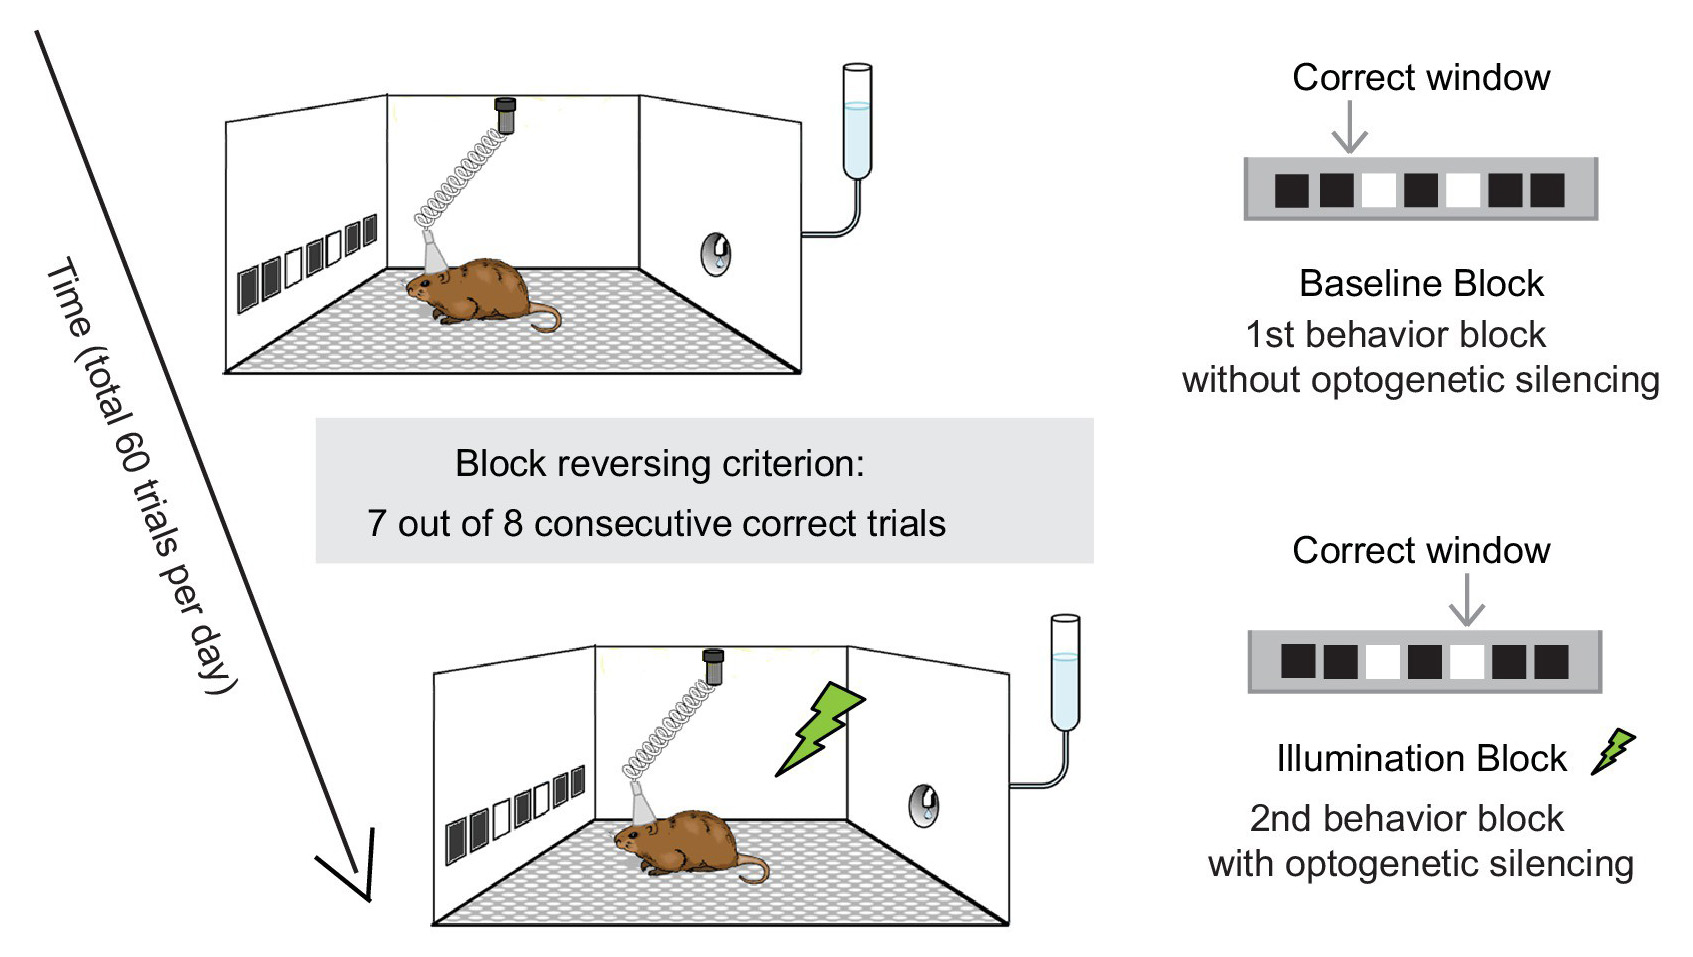
\includegraphics[width=0.5\textwidth,height=\textheight]{img/behavior-box/task-schematic.jpg}
\caption{behaviorbox schematic}
\end{figure}

\hypertarget{sec:ir-touchscreen}{%
\subsection{IR Touchscreen}\label{sec:ir-touchscreen}}

The IR touchscreen provided a robust measure of the location of any
contact with the animal's paws or nose. The screen was more reliable
than either \emph{resistive} or \emph{capacitive} touchscreens, which
are much more common in devices like POS systems and mobile phones
respectively.

Files in this folder are used to run our ``BehaviorBox'' system, which
features easily customizable control of experiments involving an
infrared touchscreen and LCD display along with speakers, water-ports,
lights, essentially anything that can be controlled electronically.

COGENT 2000 The graphics/visual-stimulation package used is missing from
this folder due to size, but can be downloaded from the
\href{http://www.vislab.ucl.ac.uk/cogent_2000.php}{source}

\hypertarget{sec:framesynx-toolbox}{%
\subsection{FrameSynx Toolbox}\label{sec:framesynx-toolbox}}

The FrameSynx toolbox for MATLAB was built to synchronize continuous
image acquisition with experiments conducted in the neuroscience
laboratory setting. While the experiments are conducted in separate
software (and potentially on a different computer), FrameSynx listens
for messages to start/stop the experiment, start a trial, etc. and
responds accordingly by controlling one or multiple cameras and
illumination devices, and synchronizing this information with the data
acquired. The major contribution to the ``Behavior Box'' package, and
also to later image processing packages is the procedure for definition
and storage and of experimental data files, which will be touched on
briefly in sec.~\ref{sec:data-file}

\hypertarget{sec:using-computer-vision-to-track-position-and-orientation}{%
\subsection{Using Computer Vision to track Position and
Orientation}\label{sec:using-computer-vision-to-track-position-and-orientation}}

\hypertarget{mouse-in-a-bowl}{%
\subsection{Mouse in a Bowl}\label{mouse-in-a-bowl}}

A webcam-based motion tracking box constructed to analyze the movement
of our unilaterally lesioned PD mouse model. Video is recorded at 15
frames per second and processed on-line or off-line using a function
written in MATLAB. Briefly, this function converts each frame to a black
and white image (logical matrix), uses morphological filtering functions
to isolate the mouse (remove mouse excrement) and identify its body
(remove the tail), then finds the center of mass in cartesian
coordinates (maximum center of projection on x- and y-axes), and the
rostral-caudal orientation measured in degrees off the x-axis.
Orientation is determined by the index of maximum of a radon transform
of the binary image. Processing is accomplished at a rate of 15-16 fps,
using a single core, or 64 fps using parallel processing on a quad-core
processor with multi-threading enabled. The advantage of this apparatus
over the virtual-reality system is that it allows free movement of an
untrained mouse, with real-time movement metrics at nearly the same rate
as the spherical treadmill.

\begin{figure}
\centering

\subfloat[Raw frame of video being
tacked]{\includegraphics[width=0.3\textwidth,height=\textheight]{img/animal-tracking/01raw.jpg}}
\subfloat[Area of detected
mouse]{\includegraphics[width=0.3\textwidth,height=\textheight]{img/animal-tracking/02black-and-white.jpg}}
\subfloat[Overlay of 3 consecutive frames showing movement of mouse
between
each]{\includegraphics[width=0.3\textwidth,height=\textheight]{img/animal-tracking/03twoframes.jpg}}

\subfloat[video overlay showing tracked
points]{\includegraphics[width=0.2\textwidth,height=\textheight]{img/animal-tracking/07mousedata1close.jpg}}
\subfloat[video overlay showing tracked
points]{\includegraphics[width=0.2\textwidth,height=\textheight]{img/animal-tracking/06mousedata1.jpg}}
\subfloat[video overlay showing tracked
points]{\includegraphics[width=0.2\textwidth,height=\textheight]{img/animal-tracking/08mousedata2.jpg}}
\subfloat[video overlay showing tracked
points]{\includegraphics[width=0.2\textwidth,height=\textheight]{img/animal-tracking/09mousedata1fiberon1.jpg}}

\caption{Automated animal Tracking for ``Mouse in a bowl'' type
experiments}

\label{fig:mouse-in-a-bowl}

\end{figure}

\hypertarget{spherical-treadmill}{%
\subsection{Spherical Treadmill}\label{spherical-treadmill}}

A virtual reality system was assembled, adopting methods from the Harvey
lab lab (Harvey et al. 2009). This system allows placement of a
head-restrained mouse on an 8-inch diameter polystyrene foam ball
supported by a cushion of compressed air, surrounded by a toroidal
projection screen. Ball rotation is tracked with two optical computer
mice placed orthogonal to each other. Movement vectors are fed into a
virtual-reality engine that updates the image projected onto a toroidal
screen surrounding the ball, simulating movement through any arbitrary
virtual world. Movement vectors are recorded as an arbitrarily scaled
translation in the mouse-relative X and Y axes and rotation around the Z
axis, at approximately 30 ms intervals. This behavioral apparatus has
the advantage of allowing trivial measurement of the mouse's movement
ability while the mouse is head-fixed. The disadvantage is the time and
potential confounds involved with training individual mice to use the
system.

\begin{figure}
\centering

\subfloat[01-treadmill-mouse-running]{\includegraphics[width=0.3\textwidth,height=\textheight]{img/spherical-treadmill-VR/01-treadmill-mouse-running.jpg}}
\subfloat[01-water-port]{\includegraphics[width=0.3\textwidth,height=\textheight]{img/spherical-treadmill-water-delivery/01-water-port.jpg}}
\subfloat[03-water-delivery-zoom]{\includegraphics[width=0.3\textwidth,height=\textheight]{img/spherical-treadmill-water-delivery/03-water-delivery-zoom.jpg}}

\caption{Spherical treadmill}

\label{fig:spherical-tradmill}

\end{figure}

\hypertarget{headplate-holder}{%
\subsection{Headplate Holder}\label{headplate-holder}}

\begin{figure}
\centering

\subfloat[front]{\includegraphics[width=0.3\textwidth,height=\textheight]{img/headplate-holder/photo-front.jpg}}
\subfloat[top]{\includegraphics[width=0.3\textwidth,height=\textheight]{img/headplate-holder/photo-top.jpg}}
\subfloat[bottom]{\includegraphics[width=0.3\textwidth,height=\textheight]{img/headplate-holder/photo-bottom.jpg}}

\caption{Headplate holder}

\label{fig:headplate-holder}

\end{figure}

\hypertarget{motion-sensors}{%
\subsection{Motion Sensors}\label{motion-sensors}}

Motion sensing was implemented using a linux computer and standard mice
at first, and later using precision laser navigation sensors for
``gaming'' mice and custom firmware written to work with any
arduino-compatible microcontroller.

\hypertarget{generic-usb-computer-mouse-with-minimal-linux}{%
\subsection{Generic USB Computer Mouse with Minimal
Linux}\label{generic-usb-computer-mouse-with-minimal-linux}}

Run ``mouse\_relay.py'' on any computer running linux to send xy-data
from 2 USB optical computer mice to another computer over an RS-232
serial-port connection. The receiving computer (in this implementation)
uses MATLAB to read the values and translate the xy-values from 2 mice
on the surface of a sphere into 3 values corresponding to rotation of
that sphere around 3 orthogonal axes (XYZ) with their origin at the
sphere's center.

RECEIVING FUNCTIONS: The MATLAB class that receives the serial input
(xy-values from both mice) is called ``VrMovementInterface''

The MATLAB function that translates the double-stream of xy-values from
the sphere's surface into rotation around its center is called
``moveBucklin.m'' and is located in the VIRMEN ``movements'' folder.

SERIAL FORMAT: XY-Values are transmitted in `packets' using an ascii
formatted string terminated by a newline. Each packet contains the
Sensor Number (s) that the reading is coming from, followed by the
X-Value (dx), then the Y-Value (dy). The python code looks like the
following:

\begin{Shaded}
\begin{Highlighting}[]
\OperatorTok{>}\NormalTok{ datastring }\OperatorTok{=}\NormalTok{ s }\OperatorTok{+} \StringTok{'x'}\OperatorTok{+}\NormalTok{dx }\OperatorTok{+} \StringTok{'y'}\OperatorTok{+}\NormalTok{dy }\OperatorTok{+} \StringTok{'}\CharTok{\textbackslash{}n}\StringTok{'}
\end{Highlighting}
\end{Shaded}

A single reading is received at the other end of the serial connection
looking something like the following:

\begin{quote}
s1x34y-3
\end{quote}

\hypertarget{navigation-sensor-chip-with-arduino}{%
\subsection{Navigation Sensor Chip with
Arduino}\label{navigation-sensor-chip-with-arduino}}

The system was later improved. Works with ADNS library to pass
{[}dx,dy{]} measurements from two ADNS-9800 laser mouse sensors (placed
45-degrees apart on surface of styrofoam ball).

\begin{figure}
\centering

\subfloat[01-motion-sensors-installed]{\includegraphics[width=0.3\textwidth,height=\textheight]{img/spherical-treadmill-motion-sensors/01-motion-sensors-installed.jpg}}
\subfloat[02-motion-sensors]{\includegraphics[width=0.3\textwidth,height=\textheight]{img/spherical-treadmill-motion-sensors/02-motion-sensors.jpg}}
\subfloat[Striatum\_Figure2]{\includegraphics[width=0.3\textwidth,height=\textheight]{img/spherical-treadmill-motion-sensors/Striatum_Figure2.png}}

\caption{Motion sensors}

\label{fig:motion-sensors}

\end{figure}

\hypertarget{microscopes}{%
\section{Microscopes}\label{microscopes}}

This section describes the background in microscopy in the
neurosciences, and also how it relates to imaging in healthcare and
electrophysiology in neuroscience. It will also describe the basic
elements necessary for the construction of a microscope in a laboratory
where calcium imaging in an animal is available. It will also refer to
later sections which cover the design and construction of mechanical
elements for animal handling and optical access (i.e.~the headplate and
a chronic optical window).

\hypertarget{background-brain-imaging-and-microscopy-in-neuroscience}{%
\subsection{Background: Brain Imaging and Microscopy in
Neuroscience}\label{background-brain-imaging-and-microscopy-in-neuroscience}}

Optical imaging has traditionally involved wide-field imaging or two
photon imaging, each with their own distinctive advantages and
disadvantages. In recent years, two photon microscopy has been a
preeminent choice for imaging in tissue, because of its high spatial
resolution, and tissue penetrating features. Two photon calcium imaging
has been broadly applied to individual cells or subcellular components
of neurons including spines and axons.

Because two photon microscopy uses a scanning mechanism, the signal to
noise ratio is influenced by the time spent imaging each point, and the
spatial resolution is determined by the number of points scanned to
obtain each image. As a result, the size of the imaging field is
inversely correlated with the overall temporal resolution while
maintaining a relatively high signal-to-noise ratio, thus, two photon
calcium imaging is often performed on a small area or on a sparse
network of cells, when dynamic responses with high temporal fidelity is
necessary.

Wide-field imaging has been used in various forms for several decades
and was first used to characterize the functional architecture and
hemodynamic responses in brain tissue. However, this technique has seen
a renaissance recently due to its simple instrumentation, relatively
inexpensive cost, and the improvements in neural signal indicators.
Optical imaging and two photon microscopy have traditionally been
performed in head-fixed preparations, but recent advances have also made
it possible to perform wide-field calcium imaging in freely moving
animals, through miniaturized and wearable microendoscope systems

While wide-field imaging lacks the spatial resolution to resolve fine
subcellular structure or the penetrating properties available with
two-photon, it is possible to obtain clear neurites and somatic
features, including spike detection

Because a single photon microscope does not rely on scanning features,
it can be used to sample a larger field of view without sacrificing
sampling rates. Additionally, recording sessions may be less sensitive
to fluorophore bleaching than other techniques, which makes it possible
to perform sustained illumination and subsequent imaging for an extended
period of time - a desired feature for analyzing neural networks during
some behavior paradigms (e.g., repeated trial learning paradigms). Thus,
wide-field imaging offers an advantage if the objective is to
simultaneously recording hundreds of neurons in the brain of a living
and behaving animal with high temporal fidelity.

\hypertarget{cameras-for-widefield-microscopy}{%
\subsection{Cameras for Widefield
Microscopy}\label{cameras-for-widefield-microscopy}}

Traditional widefield microscope or macroscope builds incorporate
`scientific grade' cameras. Compared to cameras built for other markets
(e.g.~consumer, industrial, studio, etc.), these cameras are often well
tested and certified to offer low or well-characterised noise at
moderate speeds, and a linear photo-response profile. Unlike consumer or
studio cameras which are invaribaly configured for RGB color, they are
preferably configured with `monochrome' sensors - essentially identical
to the analagous color sensor, without the bayer filter. Of much greater
importance, one must consider the unique connectivity and control
interface that scientific cameras come with. Standards exist, but are
typically unique to this segment of the industry, with poorly defined
specifications for translation to other electronic communication and
connection interface standards, such as those used in studio and
broadcast video, or those used with consumer cameras. The trait that is
the most worthy of consideration, however, is the cost. See
({\textbf{???}}) for details.

The in-vivo instrinsic-signal or fluorescent-dye imaging camera of 1
decade ago had a 0.5``-1'' monochrome CCD sensor with 0.1-1 MegaPixels,
a large well-depth, and moderately low noise at speeds around 30 to 60
fps. Connection was often LVDS, with custom electrial connectors unique
to each camera. A particularly popular and long-running model was the
Dalsa 1M30, followed by the 1M60 in later years (Takahashi et al. 2006).

\hypertarget{microscope-construction}{%
\subsection{Microscope Construction}\label{microscope-construction}}

\begin{figure}
\centering

\subfloat[Schematic showing relation of microscope and mouse on
spherical
treadmill]{\includegraphics[width=0.3\textwidth,height=\textheight]{img/microscope/widefield_microscope_diagram.png}}
\subfloat[Setup 1: the LED used for excitation can be seen extending to
the left (black covering to block
light)]{\includegraphics[width=0.3\textwidth,height=\textheight]{img/microscope/setup1.jpg}}

\caption{Basic configuration for a widefield epifluorescence microscope
for in-vivo imaging. This first configuration used a phase contrast lens
borrowed from an inverted microscope (not recommended).}

\label{fig:widefield-microscope1}

\end{figure}

\begin{figure}
\centering

\subfloat[setup3:
front]{\includegraphics[width=0.25\textwidth,height=\textheight]{img/microscope/setup3-front.jpg}}
\subfloat[setup3:
closeup]{\includegraphics[width=0.4\textwidth,height=\textheight]{img/microscope/setup3-closeup.jpg}}
\subfloat[setup3:
side]{\includegraphics[width=0.25\textwidth,height=\textheight]{img/microscope/setup3-side.jpg}}

\subfloat[setup4:
front]{\includegraphics[width=0.25\textwidth,height=\textheight]{img/microscope/setup4-front.jpg}}
\subfloat[setup4:
closeup]{\includegraphics[width=0.4\textwidth,height=\textheight]{img/microscope/setup4-closeup.jpg}}
\subfloat[setup4:
side]{\includegraphics[width=0.25\textwidth,height=\textheight]{img/microscope/setup4-side.jpg}}

\caption{Widefield fluorescence microscope reconfigured. Multiple
iterations are shown, with later iterations offering improved
compatibility with usage of off-the-shelf components.}

\label{fig:widefield-microscope3}

\end{figure}

\hypertarget{neural-signals-computational-considerations-interpretation-and-usage}{%
\chapter{Neural Signals: Computational considerations, interpretation
and
usage}\label{neural-signals-computational-considerations-interpretation-and-usage}}

\hypertarget{image-processing}{%
\section{Image Processing}\label{image-processing}}

The entire procedure for processing images and extracting cell signals
can be performed in substantially less time than most commonly available
tools using the approach described in Aim 1, particularly the methods
for restricting the spatial extent of pixel-association operations, and
distributing operations across parallel processing cores using a Single
Program Multiple Data (SPMD) archetype. However, the total time still
exceeds that of the acquisition session. Inefficiency arises from the
overhead involved with distributing data and passing information between
separate parallel processes. Graphics cards, however execute in what's
called Single Instruction Multiple Data (SIMD) fashion, to distribute
computation across the thousands of processing cores.

The processing components are implemented using the MATLAB System-Object
framework, which allows for slightly faster performance through internal
optimizations having to do with memory allocation. Most system objects,
each representing one step in the serial processing and
signal-extraction procedure, also have companion functions that
implement the computation-heavy components of each algorithm using a
pre-compiled CUDA kernel.

\hypertarget{benchmarking-general-performance}{%
\subsection{Benchmarking \& General
Performance}\label{benchmarking-general-performance}}

Built-in MATLAB functions that execute on the GPU can be profiled with
benchmarking functions like \emph{gputimeit()}, or with the
\emph{tic/toc} functions. When execution isn't fast enough, they need to
be replaced with custom functions. The custom functions typically
achieve the speed up necessary by enabling the operation to carried out
on several frames at once. This reduces the over-head costs inposed for
each function call by spreading it over several frames. This solution is
not ideal, as it increases the latency of solutions, however does not
preclude implementation in real-time system if the procedures are
adapted to run on a real-time hybrid system-on-module like NVIDIA's
Tegra X1, which should involve minimal effort once a standard set of
successful procedures is realized. The current implementation tests the
processing time of each stage of the process to ensure that the sum is
less than the acquisition time for each frame dictated by the inverse of
the frame-rate (30-50 milliseconds).

\hypertarget{buffered-operations}{%
\subsection{Buffered Operations}\label{buffered-operations}}

Combining frames for each operation can result in near linear speedup.
For example, for the phase-correlation step required for motion
correction, the FFT and IFFT are called on 16 image-frames at once, and
the time take to accomplish is approximately the same as if the
operation were called on 1 frame. This essentially leads to a 16x
speedup, though the latency is also increased slightly. The best size to
use is difficult to pre-determine, and typically must be measured for
varying size `chunks' using the benchmarking functions indicated above.
The system objects manage the details necessary to allow buffered chunks
of video to be passed to each stage without introducing artifacts at the
temporal edges between chunks.

\hypertarget{image-pre-processing-motion-correction}{%
\subsection{Image Pre-Processing \& Motion
Correction}\label{image-pre-processing-motion-correction}}

Pre-processing is implemented as with the offline procedure, with a few
changes. Images are aligned in chunks, and they are aligned sequentially
to two templates. One template is the most recent stable frame from the
preceding chunk. The other is a recursively temporal-low-pass filtered
image that mitigates slow drifts. Aligning to the first template is
usually more stable as the brightness of cells in the recent image will
be more similar to those in the current chunk than will be the
brightness of cells in the slow-moving average.

The displacement of each frame is found to sub-pixel precision, then
used with a custom bicubic resampling kernel that replaces any pixels at
the edges with images from the moving average.

\hypertarget{sequential-statistics}{%
\subsection{Sequential Statistics}\label{sequential-statistics}}

A number of statistics for each pixel are updated online and can be used
for normalization and segmentation procedures later in the process.
These include the minimum and maximum pixel intensity, and the first
four central moments, which are easily converted to the mean, variance,
skewness, and kurtosis. The formulas for making these calculations are
given below, and are performed in a highly efficient manner as data are
kept local to each processing core, and repeat computations are
minimized.

\begin{Shaded}
\begin{Highlighting}[]
\NormalTok{n = n + }\FloatTok{1}\NormalTok{;}
\NormalTok{f = F(rowIdx,colIdx,k);}
\NormalTok{d = single(f) - m1;}
\NormalTok{dk = d/n;}
\NormalTok{dk2 = dk\textbackslash{}^}\FloatTok{2}\NormalTok{;}
\NormalTok{s = d\textbackslash{}*dk\textbackslash{}*(n-}\FloatTok{1}\NormalTok{);}

\CommentTok{% UPDATE CENTRAL MOMENTS}
\NormalTok{m1 = m1 + dk;}
\NormalTok{m4 = m4 + s\textbackslash{}*dk2\textbackslash{}*(n.\textbackslash{}^}\FloatTok{2}\NormalTok{-}\FloatTok{3}\NormalTok{\textbackslash{}*n+}\FloatTok{3}\NormalTok{) + }\FloatTok{6}\NormalTok{\textbackslash{}*dk2\textbackslash{}*m2 - }\FloatTok{4}\NormalTok{\textbackslash{}*dk\textbackslash{}*m3;}
\NormalTok{m3 = m3 + s\textbackslash{}*dk\textbackslash{}*(n-}\FloatTok{2}\NormalTok{) - }\FloatTok{3}\NormalTok{\textbackslash{}*dk\textbackslash{}*m2;}
\NormalTok{m2 = m2 + s;}

\CommentTok{% UPDATE MIN & MAX}
\NormalTok{fmin = min(fmin, f);}
\NormalTok{fmax = max(fmax, f);}
\end{Highlighting}
\end{Shaded}

Furthermore, the value used to update each central moment at each point
in time can be used as a measure of change in the distribution of each
pixel caused by the current pixel intensity, as explained next.

\hypertarget{non-stationarity-differential-moments}{%
\subsection{Non-Stationarity \& Differential
Moments}\label{non-stationarity-differential-moments}}

Stationary refers to the property of a signal such that its statistics
do not vary over time, i.e.~its distribution is stable. Neural signals
tend to specifically \emph{not} have this property, in contrast to other
measurable components such as those contributed by physiologic noise
(heart-rate, respirations, etc.). Thus, by analyzing the evolution of
statistical measures calculated for each pixel as frames are added in
sequence gives a highly sensitive indicator of neural activity. This is
done using a routine analogous to that for updating central moments
given above, except the values returned are not only the updated moment,
but also the updating component -- essentially the partial derivative
with respect to time. This is illustrated below, including the
normalization functions which convert the partial-moment values to their
variance, skewness, and kurtosis analogues:

\begin{Shaded}
\begin{Highlighting}[]
\NormalTok{dm1 = dk;}
\NormalTok{m1 = m1 + dm1;}
\NormalTok{dm4 = s\textbackslash{}*dk2\textbackslash{}*(n\textbackslash{}^}\FloatTok{2}\NormalTok{-}\FloatTok{3}\NormalTok{\textbackslash{}*n+}\FloatTok{3}\NormalTok{) + }\FloatTok{6}\NormalTok{\textbackslash{}*dk2\textbackslash{}*m2 - }\FloatTok{4}\NormalTok{\textbackslash{}*dk\textbackslash{}*m3;}
\NormalTok{dm3 = s\textbackslash{}*dk\textbackslash{}*(n-}\FloatTok{2}\NormalTok{) - }\FloatTok{3}\NormalTok{\textbackslash{}*dk\textbackslash{}*m2;}
\NormalTok{dm2 = s;}
\NormalTok{m2 = m2 + dm2;}
\NormalTok{dm2 = dm2/max(}\FloatTok{1}\NormalTok{,n-}\FloatTok{1}\NormalTok{);}
\NormalTok{dm3 = dm3\textbackslash{}*sqrt(max(}\FloatTok{1}\NormalTok{,n))/(m2\textbackslash{}^}\FloatTok{1.5}\NormalTok{);}
\NormalTok{dm4 = dm4\textbackslash{}*n/(m2\textbackslash{}^}\FloatTok{2}\NormalTok{);}
\end{Highlighting}
\end{Shaded}

Caption: Differential-update-to-central-moments

These functions run on images representing the image intensity, and also
on images taken from sequential differences indicating the temporal
derivative of image intensity. The combination of outputs from these
operations indicate both when image intensities are significantly high
relative to past distribution, and also when intensities are changing
significantly faster than learned from their past distribution.

\hypertarget{surface-classification-peaks-edges-curvature}{%
\subsection{Surface Classification: Peaks, Edges,
Curvature}\label{surface-classification-peaks-edges-curvature}}

Edge-finding methods are employed for establishing boundaries between
cells, and first and second-order gradients are used to compute local
measures of curvature from an eigenvalue decomposition of the local
Hessian matrix. I won't go into detail, as the utility of these
procedure in the most recent implementation has been lost, but
nevertheless, the operation is optimized and ready to be plugged back in
when further development calls for better accuracy informing
cell-segmentation, or when a faster or more accurate motion-correction
algorithm is called for.

\hypertarget{online-cell-segmentation-tracking}{%
\subsection{Online Cell Segmentation \&
Tracking}\label{online-cell-segmentation-tracking}}

Cells are segmented by first running sequential statistics on the
properties of identifiable regions on a pixel-wise basis. That is, as
regions are identified in a method similar to that used offline in Aim
1, the region-properties are calculated (Centroid, Bounding-Box, etc.)
and statistics for these properties are updated at each pixel covered by
a proposed region. After sufficient evidence has gathered, Seeds are
generated by finding the local peak of a seed-probability function that
optimizes each pixel's proximity to a region centroid, and distance from
any boundary. Regions are grown from these seed regions, and registered
in a hierarchy that allows for co-labeling of cellular and sub-cellular
components. Newly identified regions occur as new seeds, where as seeds
overlapping with old regions are used to identify sub-regions, or to
track regions over time.

\hypertarget{signal-extraction-from-subcellular-compartments}{%
\subsection{Signal Extraction from Subcellular
Compartments}\label{signal-extraction-from-subcellular-compartments}}

I also have functions for the extraction of normalized
Pointwise-Mutual-Information (nPMI), which can operate on a
pixel-to-pixel basis or on a region-to-pixel basis. This operation
accumulates mutually informative changes in all pixels in the maximal
bounding-box (e.g.~64x64 pixels) surrounding each identified regions
centroid. The weights given by this function can take on values between
-1 and 1, and can be used to inform any reduction operations to follow.
Additionally, spatial moments can indicate the subcellular distribution
of activity across the identified region. In this context, the first
spatial moment M\textsubscript{00} indicates the mean signal intensity.

\hypertarget{user-interface-for-parameter-tuning}{%
\subsection{User Interface for Parameter
Tuning}\label{user-interface-for-parameter-tuning}}

Some system-objects also incorporate a user interface to aid in
parameter selection for tuning.

\hypertarget{image-processing-tonemapping-and-filtering}{%
\subsection{Image Processing: Tonemapping and
Filtering}\label{image-processing-tonemapping-and-filtering}}

\begin{figure}
\centering
\includegraphics[width=0.5\textwidth,height=\textheight]{img/sw-gui-interactive-parameter-selection-homomorphic-filter/Screenshot_20150608180058.png}
\caption{interactive parameter selection for homomorphic filter}
\end{figure}

\begin{figure}
\centering
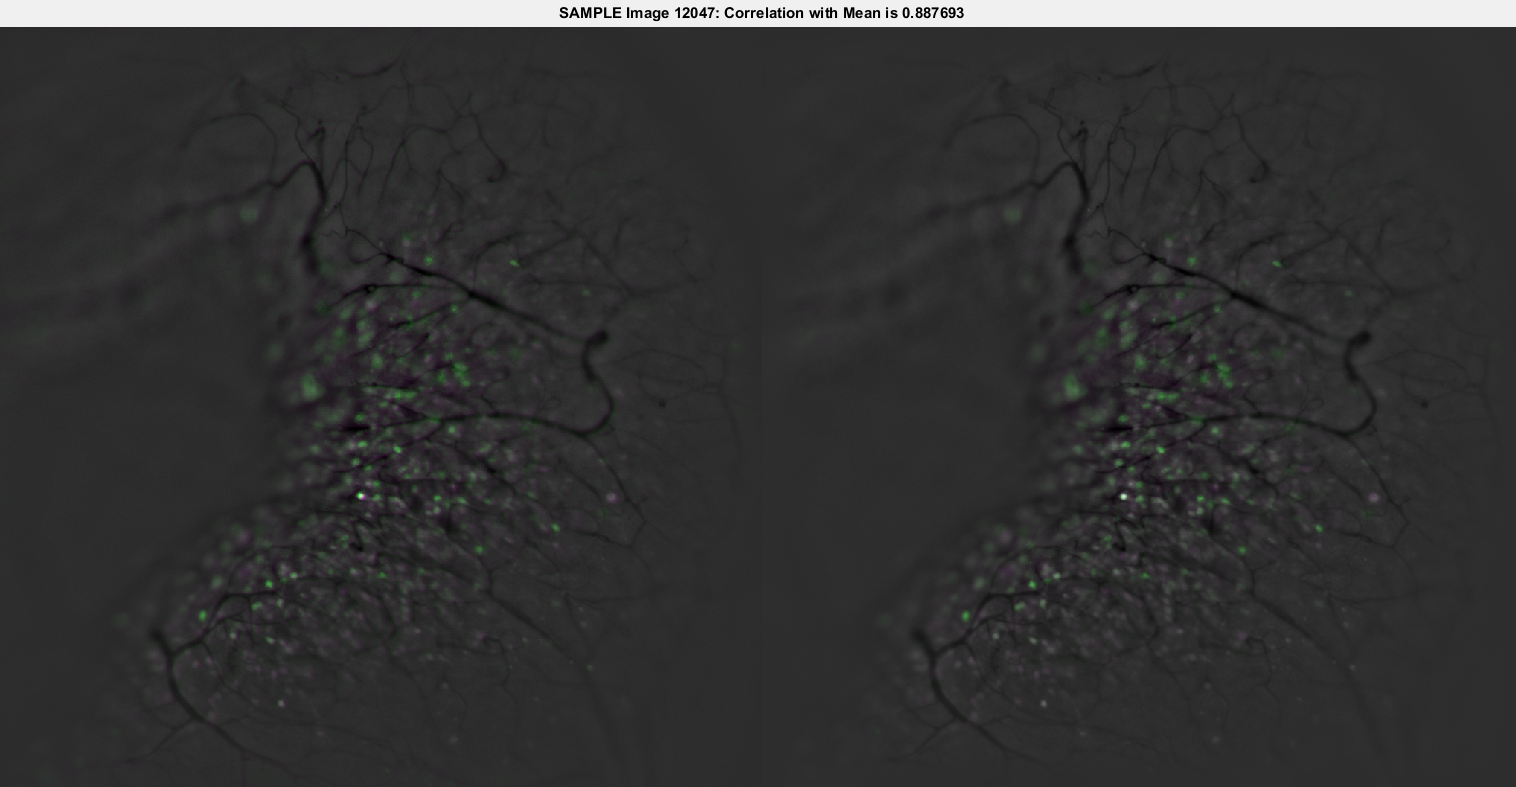
\includegraphics[width=0.5\textwidth,height=\textheight]{img/sw-fluopro/motion_correction_sample.png}
\caption{motion Correction}
\end{figure}

\begin{figure}
\centering
\includegraphics[width=0.5\textwidth,height=\textheight]{img/sw-video-processing-feature-generation.png}
\caption{feature generation}
\end{figure}

\begin{figure}
\centering
\includegraphics[width=0.5\textwidth,height=\textheight]{img/2.png}
\caption{Pixel features useful for segmentation}
\end{figure}

\begin{figure}
\centering
\includegraphics[width=0.5\textwidth,height=\textheight]{img/sw-video-processing-feature-pointwise-mutual-information.png}
\caption{using limited spatiotemporal information for fast pixel-wise
feature generation, in this case Pointwise Mutual Information (PMI)}
\end{figure}

\begin{figure}
\centering
\includegraphics[width=0.5\textwidth,height=\textheight]{img/sw-sequence-bw.png}
\caption{pixel statistics}
\end{figure}

\begin{figure}
\centering
\includegraphics[width=0.5\textwidth,height=\textheight]{img/trgb-013.png}
\caption{pixel-wise labeling: assignment of each pixel to cellular
regions of interest overlayed on pixel intensity}
\end{figure}

\begin{figure}
\centering
\includegraphics[width=0.5\textwidth,height=\textheight]{img/sw-video-statistics/statistics_of_128_frames_contrast_enhanced.jpg}
\caption{central moments}
\end{figure}

\hypertarget{discussion-the-last-mile-in-computing-for-clinicians-engineers-and-research-scientists}{%
\chapter{Discussion: the last mile in computing for clinicians,
engineers, and research
scientists}\label{discussion-the-last-mile-in-computing-for-clinicians-engineers-and-research-scientists}}

This dissertation has presented straightforward methods for assembling
laboratory equipment that can capture the behavior and neural activity
of laboratory animals, and procedures for managing and making use of the
collected data. In some ways the recommended procedures may deviate from
standard practice or what may jump forth as the most obvious approach.
The \textbf{why} is what I wish to address here.

\hypertarget{state-of-current-methods}{%
\section{State of current methods}\label{state-of-current-methods}}

At the start of the work described here we found ourselves with
technology providing ``neural signals'' that vastly exceeded our
expectations and the assumptions of the tools we applied to work with
it. In the past, fluctations in optical imaging data were dominated by
``noise.'' The form of noise depended on the process; all types of
imaging, intrinsic signal, fluorescent dye, etc., had relatively small
fluctuations resulting from neural activity. With new engineered
molecules, like GCaMP6, and new images sensors, like those dubbed
\textbf{scientific CMOS}, these sources of noise become relatively
small. The large change in signal-to-noise ratio opens the door for new
opportunities and change to traditional routines. The abundance of
signals available from our research animals not only makes old routines
\textbf{inefficient}, but paradoxically \textbf{insufficient}. Such an
abundance of factors at our finger tips requires a level of discipline
in study design to make the scientific method work that was previously
unneccessary, as the difficulty in finding signals was inherently self
regulating.

\hypertarget{signal-and-noise-in-neural-imaging-data}{%
\subsection{Signal and Noise in Neural Imaging
Data}\label{signal-and-noise-in-neural-imaging-data}}

Traditional noise in neural signals can be roughly categorized as having
origin in physiology or technology. The physiological noise sources
would include ``artifacts'' caused by an animal's breathing, the beats
of their heart, or the movement they make as they react to the
experimentally controlled world around them. Technological noise is
usually broken down into sensor noise sources, \textbf{read noise} and
\textbf{thermal noise}, and noise relating to digitization. A third type
of ``noise'' could arguably be categorized as either, as it lies at the
interface of technology and biology, for example the complex
interactions of exogenous calcium-binding proteins like GCaMP with the
endogenous calcium handling proteins of a neuron. By a strict
definition, however, only the sensor noise should really be called
\textbf{noise}, as other sources are not entirely unpredictable. They
can be accounted for.

At any rate, the level of noise in the signals gathered by a combination
of GCaMP6 and a sCMOS camera is miniscule relative to the signals
indicating fluctuation in calcium concentration. The problem of
visualization of these signals remains, however, as the dynamic range of
signal varies tremendously over space and time, and requires some
treatment prior to display on our currently limited computer monitors.
Previously common methods, particularly intrinsic-signal imaging,
provided very small signals that required averaging over time before any
response could be ascertained.

\hypertarget{correlation-confounding-signals-and-non-linear-dyanamics}{%
\subsection{Correlation, Confounding Signals, and Non-linear
dyanamics}\label{correlation-confounding-signals-and-non-linear-dyanamics}}

\hypertarget{motion-artifact}{%
\subsection{Motion Artifact}\label{motion-artifact}}

\hypertarget{exponential-expansion-in-data-volume}{%
\section{Exponential Expansion in Data
Volume}\label{exponential-expansion-in-data-volume}}

The quality of cheaply available sensors has risen drastically. These
new sensors are everywhere. They are quick to interface with, and the
stream of information they provide once switched on is unlimited. In the
starkest contrast, however, storage for this never-ending stream of data
is both finite in its capacity, and cumulative in consumption.

\hypertarget{fields-sharing-this-problem}{%
\subsection{Fields sharing this
problem}\label{fields-sharing-this-problem}}

Scientists all over find themselves with a lab full of sensors,
data-rich and space-poor. For better or worse they are not alone in
dealing with this problem. Massive investment has been poured into
managing this issue for commercial purposes, and -- perhaps unsettlingly
-- for governmental surveillance purposes. The volume of recordable
traffic bouncing through choke points of the internet exceeds the
capacity of any government to store for more than 24 hours or so.
Likewise, the volume of video data streaming in from video surveillance
systems as massive as those found for instance in China necessitates
similar solution to what scientists and physicians have or should expect
to deal with.

\hypertarget{technological-opportunities-to-expect}{%
\subsection{Technological Opportunities to
Expect}\label{technological-opportunities-to-expect}}

The solutions begin proposed by commercial and governemental giants are
not radical. They include calls for standardization in the format of
data, enabling solutions for efficient transmission and storage to be
shared through improvement of common tools. Common streaming formats
allow compression and storage to be abstracted from each application.
Databases are being developed to take advantage of heterogeneous
computational architectures and distributed storage spaces. Traditional
document-based or relational databases are outperformed by graph-based
``triple-store'' databases, timeseries databases, and by databases
programmed for specific architecture, like GPU-databases. These sorts of
developments are targeted at the bottlenecks restricting access to data,
and early results suggest orders of magnitude improvements in
throughput. These tools are being developed with or without the
contribution of physicians and scientists. It would be prudent however
to orient the tools specific to the needs of scientists and clinicians
to take advantage of these developments as they become available.

\hypertarget{clinical-translation-potential}{%
\section{Clinical translation
potential}\label{clinical-translation-potential}}

Any device that relies on optogenetics to deliver stimulation to neurons
inherently shares the same hurdles to clinical translation, the
requirement for gene-therapy and its associated risks. Several early
trials of viral transfection of cells had adverse effects including a
greatly increased risk of carcinoma. In these early studies, the DNA
insertion location was uncontrolled leaving important regions of DNA
tumor suppressor genes exposed to damage. New methods that improve the
safety of gene therapy have been developed. Several of the more recent
methods utilize adeno-associated virus (AAV) and show greater control
regarding DNA insertion and decreased DNA damage. These more recent
methods suggest a possibility that with continuing research, such a
method may be developed without the potential for malignancy.

Working on a project that requires a technology that does not as of yet
exist, represents one of the greatest educational benefits of this
project. That leap of faith into a future that does not exist requires
us to depend on each other as a team of collaborators, as each of our
work depends on the others' success. In order to succeed, we must do so
together; and without eachother, our therapeutics would never reach
their ultimate goal, the patient. As such, we would share each success
and setback in the same way whether such events occur within our own
labs or labs across the country.

\hypertarget{cranial-window}{%
\section{Cranial Window}\label{cranial-window}}

The two-stage cranial implant device described here was developed to
enable reliable long-term optical access and intermittent physical
access to mouse neocortex. Our particular application required bilateral
cortical windows compatible with wide-field imaging through a
fluorescence microscope, and physical access to the underlying tissue
for virus-mediated gene delivery and injection of exogenous labeled
cells. Optical access was required as soon as possible
post-installation, and to be sustained for several months. The design
focused on addressing the issue common to other window designs meant for
rodents: progressive degradation of the optical light-path at the
brain-to-window interface caused by highly scattering tissue growth. The
elastomer insert is molded to fit the chamber and craniotomy, blocking
tissue growth and providing a reliable optical interface for up to one
year. Additionally, the core design can be rapidly adapted to improve
performance or for varying applications.

\hypertarget{critical-elements}{%
\subsection{Critical Elements}\label{critical-elements}}

In assessing the design presented here, we can point to a few critical
elements that facilitate the maintenance of the long-term optical
quality. Refer to the methods section for the specifics of surgical
procedures for headplate installation and insert attachment. These
procedures were established after testing the variable formulations in
protocol.

First, the design of the silicone insert must incorporate a mechanical
barrier that fits along the edges of the craniotomy. The barrier must be
continuous along the circumference, and extend as far as the inside
surface of the skull to be effective.

Achieving this tight fit without agressively impinging on the brain
requires some sort of fine height adjustment capability. The silicone
insert must be attached at the correct height during the installation
procedure, or shortly thereafter. The insert must be depressed very
slightly until full contact is made across the entire window, but
pressing beyond necessary will quickly exert an undesired increase in
intracranial pressure, increasing inflammation and adverse outcomes. The
mechanism for fine adjustment can be designed into the system, as is
demonstrated in the second design presented here, or incorporated into
the installation procedure, as is done in the first design.

Of particular note, we found that administration of antibiotic and
anti-inflammatory drugs in the days surrounding any major surgical
procedure had a substantial impact on the viability of the optical
interface. We used both corticosteroid and non-steroidal
anti-inflammatory drugs, and attempts to exclude either ended poorly
more often than not.

Lastly, sealing the chamber is absolutely vital to the viability of the
optical interface, as well as health of the animal. Equally critical to
the long-term health of the imaging chamber was the requirement to
establish and maintain an air-tight seal between the chamber and the
outside world. This includes a permanent seal between the chamber and
skull, and a reversible seal between the chamber rim and optical insert.
How this is accomplished will be specific to the system design, but it
is absolutely essential.

In addition to establishing and maintaining an air-tight seal, it is
necessary to eliminate any and all pockets of air within the chamber.
Any air pockets that remain after installation will be susceptible to
bacteria growth and may disrupt normal intracranial and intermembrane
pressures. The system presented here used sterile agarose fill to
displace all air within the chamber prior to sealing. Dead space
surrounding the silicone insert, including that temporarily filled with
agarose, will fill with fluid and eventually be overtaken by granulation
tissue. This process is helpful to the maintenance of a sterile chamber
environment, so care should be taken not to disrupt it. However, an
excess of dead space will delay this process, and thus should be
minimized when adapting the design.

Many attempts to test variations from the described procedures indicated
that all elements mentioned above are equally critical to achieving a
reliable imaging window with sustained optical quality. Implementing the
procedures as described or something similar should mitigate the primary
obstacle to long-term imaging in mice and other rodents. The need to
pre-terminate imaging experiments due to light-path disruption by tissue
ingrowth should be substantially reduced. This capability will
drastically reduce wasted time and resources for experiments of any
duration, and will facilitate previously infeasible studies requiring
long-term observation such as for research in aging or the progression
chronic neurological disorders.

\hypertarget{staging-implant-installation-tissue-access}{%
\subsection{Staging Implant Installation \& Tissue
Access}\label{staging-implant-installation-tissue-access}}

Configuring the implant as described, so as to enable a staged
installation of multiple parts enables surgical procedures to be spread
across multiple days. This capability offers a number of advantages. It
may save time and resources -- particularly during the prototype stages
-- by allowing time to ensure each implanted animal fully recovers from
the initial procedure. Additionally, the delay between surgeries allows
the heightened inflammation and other immune system response triggered
by craniotomy to normalize before attempting a tissue intervention that
is sensitive to these conditions (e.g.~viral or cell injections).
Through this mechanism the system offers the capability to image the
first tissue intervention from day 0.

Similarly, designing the system to be installable in multiple stages
enables trivial and repeatable tissue access at later time points by
simple reversal of procedure for insert attachment. The process may be
comparable to a previously reported method of removing the entire glass
window to access the tissue. With this system, however, the methods used
to detach and reattach are faster and simpler and carry less risk of
tissue damage compared. Additionallly, the described methods of
facilitating tissue access can be advantageous over a fixed access port
by providing full access without compromising the image field.

\hypertarget{design-adaptation}{%
\subsection{Design Adaptation}\label{design-adaptation}}

The specific designs described in this report work well and have much to
offer; however, the greatest asset of the underlying system is its
potential for fast and unrestricted adaptation. Most users will find
greater utility in adopting components of the design and fabrication
process, customized to fit their exact needs. The design can be rapidly
transformed to accommodate various applications or to modify its
performance in response to new technologies and demands. This rapid
adaptability was a primary goal of this project, and informed our design
and engineering decisions throughout developement. Anyone with access to
common laboratory equipment and moderate engineering and fabrication
skills can produce a system to fit their particular needs. As an
inherent aspect of any design process, the adaptation of the original
design evolved over the course of prototyping and testing. In presenting
two designs in this report, our intention was to demonstrate the
technical feasibility of continuous development of a future-proof
system. The original system was adapted to accomodate the continuous
evolution of image sensor technology, particularly the growth in size
and resolution, expanding the field of view and allowing simultaneous
access to cellular interactions across multiple brain regions using
wide-field imaging.

\hypertarget{references}{%
\chapter*{References}\label{references}}
\addcontentsline{toc}{chapter}{References}

\hypertarget{refs}{}
\leavevmode\hypertarget{ref-harvey_intracellular_2009}{}%
Harvey, Christopher D., Forrest Collman, Daniel A. Dombeck, and David W.
Tank. 2009. ``Intracellular Dynamics of Hippocampal Place Cells During
Virtual Navigation.'' \emph{Nature} 461 (7266): 941--46.
\url{https://doi.org/10.1038/nature08499}.

\leavevmode\hypertarget{ref-iancu_behavioral_2005}{}%
Iancu, Ruxandra, Paul Mohapel, Patrik Brundin, and Gesine Paul. 2005.
``Behavioral Characterization of a Unilateral 6-OHDA-Lesion Model of
Parkinson's Disease in Mice.'' \emph{Behav. Brain Res.} 162 (1): 1--10.
\url{https://doi.org/10.1016/j.bbr.2005.02.023}.

\leavevmode\hypertarget{ref-ince_presence_2009}{}%
Ince, Robin A. A., Fernando Montani, Ehsan Arabzadeh, Mathew E. Diamond,
and Stefano Panzeri. 2009. ``On the Presence of High-Order Interactions
Among Somatosensory Neurons and Their Effect on Information
Transmission.'' \emph{J. Phys.: Conf. Ser.} 197 (1): 012013.
\url{https://doi.org/10.1088/1742-6596/197/1/012013}.

\leavevmode\hypertarget{ref-takahashi_vivo_2006}{}%
Takahashi, Eiji, Tomohiro Takano, Yasutomo Nomura, Satoshi Okano, Osamu
Nakajima, and Michihiko Sato. 2006. ``In Vivo Oxygen Imaging Using Green
Fluorescent Protein.'' \emph{Am. J. Physiol. - Cell Physiol.} 291 (4):
C781--C787. \url{https://doi.org/10.1152/ajpcell.00067.2006}.

\end{document}
